\documentclass{article}
\usepackage{amsmath}
\usepackage{bm}
\usepackage{graphicx}

\title{Exercise 1}
\author{Daniel Gallo}
\date{September 2020}

\begin{document}
\maketitle
\section*{18.8}
Let $Y$ be an ordered set in the order topology. Let $f,\ g \colon X \rightarrow Y$ be continuous.
\begin{enumerate}
    \item Show that the set $\left\{x \mid f(x) \leq g(x)\right\}$ is closed in X.
    \item Let $h\colon X \rightarrow Y$ be the function
    \begin{equation*}
        h(x) = min\left\{f(x),\ g(x)\right\}
    \end{equation*}
    Show that $h$ is continuous.
\end{enumerate}
\subsection*{Every order topology is Hausdorff}
First of all, we will proof that $Y$ is indeed Hausdorff. Given two elements $a,\ b \in Y$ such that $a < b$, we can consider the following set.
\begin{equation*}
    S = \left\{y \mid a < y < b\right\}
\end{equation*}
Now the following situations arise.
\begin{itemize}
    \item If S is empty, we can choose $U = \left(-\infty,\ b\right)$ and $V = \left(a,\ \infty\right)$.
    \item If there is at least one element (which we can call $c$), we can choose $U = \left(-\infty,\ c\right)$ and $V = \left(c,\ \infty\right)$.
\end{itemize}
In either case, $U$ is a neighborhood of $a$ and $V$ is a neighborhood of $b$, since open rays are open. Furthermore, their intersection is empty. We can conclude then that $Y$ is Hausdorff.
\subsection*{Proving the complement is open}
As we usually do, instead of proving that $\left\{x \mid f(x) \leq g(x)\right\}$ is closed we will prove that its complement, which we can call $W$ is open. To do so, we will show that for every $x \in W$ there exists an open set inside of $W$ containing $x$. $W$ will be open since it will be a union of open sets $W = \bigcup\limits_{x \in W}W_x$. 
\\
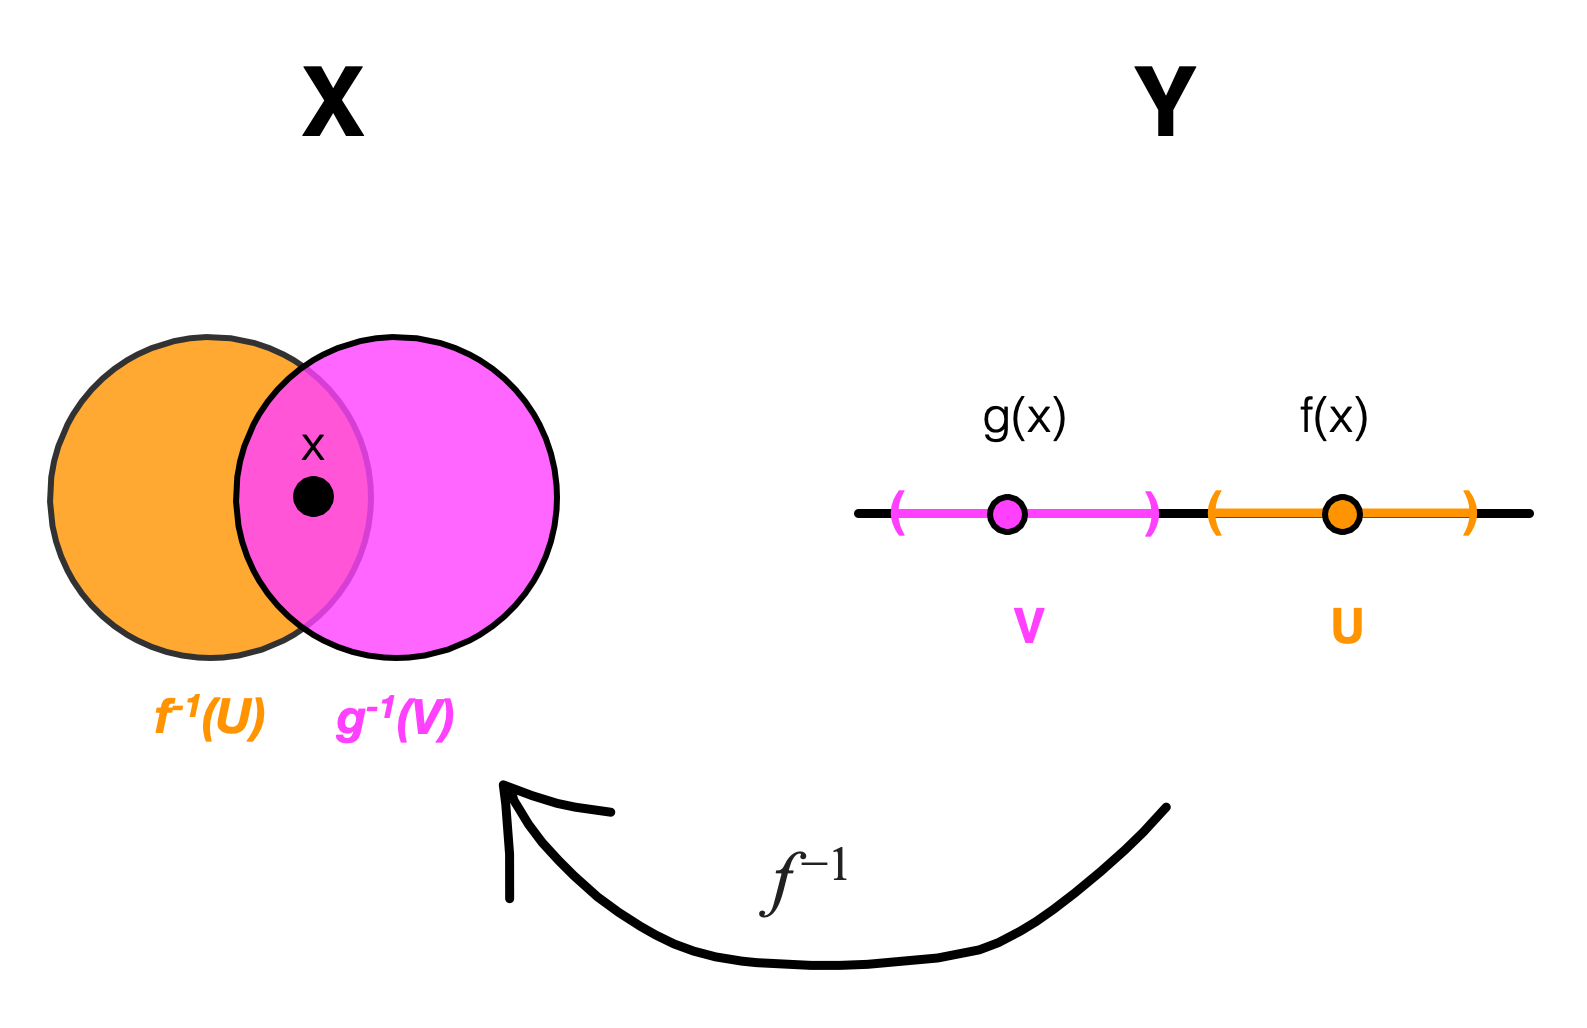
\includegraphics[width=\textwidth]{diagram.png}
Let $x \in W$, that is $f(x) > g(x)$. Since $Y$ is a Hausdorff space, there are disjoint neighborhoods of $f(x)$ and $g(x)$, $U$ and $V$. Since $f$ and $g$ are continuous functions, we know that $f^{-1}(U)$ and $g^{-1}(V)$ are open and both of them contain $x$. The intersection, $W_x = f^{-1}(U) \cap g^{-1}(V)$, will be open and nonempty, and we know that $f(x') \in U$ and $g(x') \in V$ for every $x' \in W_x$. Every element in $U$ is bigger than every element of $V$, and thus we can conclude that $W_x \in W$.
\subsection*{Proving continuity}
It is easy to see that the definition of $h$ is equivalent to this one.
\begin{equation*}
    h(x) = \left\{
        \begin{array}{ll}
        f(x) & \mathrm{if\ } x \in A = \left\{x \mid f(x) \leq g(x)\right\} \\
        g(x) & \mathrm{if\ } x \in B = \left\{x \mid g(x) \leq f(x)\right\} \\
        \end{array}
    \right.
\end{equation*}
We can now check that all conditions of the pasting lemma are satified.
\begin{gather*}
    \text{$A$ and $B$ are closed} \\
    X = A \cup B  \\
    \text{$f$ and $g$ are continuous} \\
    \forall x \in A \cap B,\ f(x) = g(x)
\end{gather*}
Thus, we can conclude that $h$ is continuous.
\section*{19.3}
If each $X_\alpha$ is a Hausdorff space, then $\prod X_\alpha$ is a Hausdorff space in both the box and product topologies.
\\
Given $\bm{a} \neq \bm{b}$, there is a $\beta$ such that $\bm{a}_\beta \neq \bm{b}_\beta$. Since $X_\beta$ is Hausdorff, we can find $U_\beta$ and $V_\beta$, neighborhoods of $\bm{a}_\beta$ and $\bm{b}_\beta$, where $U_\beta \cap V_\beta = \emptyset$. Now, we can define $U = \prod{U_\alpha}$ and $V = \prod{V_\alpha}$ as follows:
\begin{equation*}
    U_\alpha = \begin{cases}
        U_\beta  & \text{if } \alpha = \beta \\
        X_\alpha & \text{if } \alpha \neq \beta
    \end{cases}
    \qquad
    V_\alpha = \begin{cases}
        V_\beta  & \text{if } \alpha = \beta \\
        X_\alpha & \text{if } \alpha \neq \beta
    \end{cases}
\end{equation*}
$U$ and $V$ are neighborhoods of $\bm{x}$ and $\bm{y}$, and they are disjoint in both the box topology and the product topology. Since we can find a separation between different points, we can conclude that $\prod X_\alpha$ is Hausdorff.
\end{document}